
\startslide{The Name of the Game}
Multiple sensor networks from different security domains interacting.

\cemph{Example:} Time synchronization

Can a system providing policy drive authorization (trust management) be supported on such small
devices?
\begin{citemize}
\item Public key cryptography?
\item Logic program execution?
\item Symmetric key cryptography?
\end{citemize}
\stopslide

% TRUST MANAGEMENT!

\startslide{Direct Approach}

\begin{citemize}
\item Do all the computations on the nodes!
\item \cemph{SpartanRPC}: An RPC discipline for sensor networks.
\item \cemph{Sprocket}: An implementation of SpartanRPC.
\end{citemize}

Sprocket translates SpartanRPC programs into plain nesC programs.

\begin{center}
\url{https://github.com/pchapin/sprocket}
\end{center}

(paper under review at TISSEC)
\stopslide

\startslide{Dynamic Wires}
\begin{lstlisting}[language=nesC]
configuration AppC { }
implementation {
   components ClientC, SelectorC;

   activate "*" for ClientC.LEDControl ->
       [SelectorC].LEDControl;
}
\end{lstlisting}

Use all certificates available (``*'') for invocation.
\stopslide

\startslide{Duties}
\begin{lstlisting}[language=nesC]
module ServerC {
  provides remote interface LEDControl requires "A.r";
}
implementation {
  duty void LEDControl.setLEDs(uint8_t mask)
  {
    ...
  }
}
\end{lstlisting}

Server requires client to prove membership in role $A.r$.
\stopslide

\startslide{Sprocket Runtime System}
\begin{center}
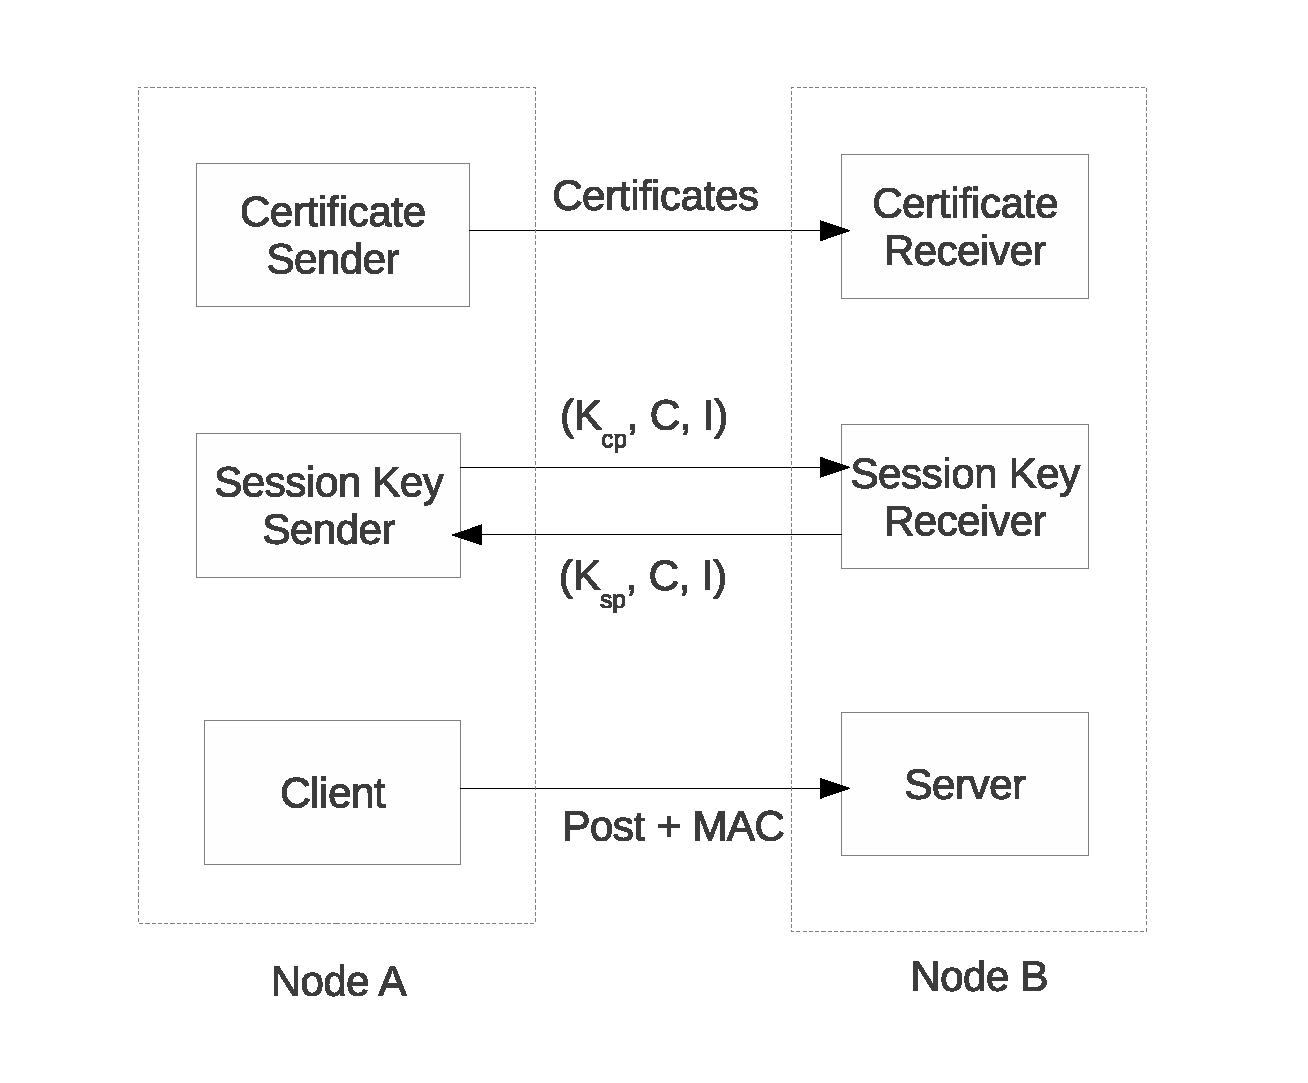
\includegraphics[scale=0.85]{SprocketRT-Protocol.eps}
\end{center}
\stopslide

\startslide{Maximum Message Transfer Rate}
\begin{center}
  \newcommand\T{\rule{0pt}{2.1ex}}
  \begin{tabular}{|l|r|r|} \hline
    \textit{Test} \T & \textit{messages/s} & \textit{\% Reduction} \\
    \hline \hline

    Baseline \T & 128 &   -- \\ \hline 
    Duties   \T & 119 &  7.0 \\ \hline
    MAC      \T &  87 & 32.0 \\ \hline
  \end{tabular}
\end{center}

The MAC was computed using hardware assisted AES on the nodes.

(Tmote Sky, 16KiB RAM, 48KiB ROM, 8MHz MSP430, TinyOS 2.1.2)
\stopslide

\startslide{Processing Time for Transient Operations}
\begin{center}
  \newcommand\T{\rule{0pt}{2.1ex}}
  \begin{tabular}{|l|r|} \hline
    \textit{Operation} \T & \textit{Time} \\ \hline \hline

    Certificate Verification     \T &  82s \\ \hline 
    Minimum Model Construction   \T & 370$\mu$s \\ \hline
    Session Key Negotiation      \T &  80s\\ \hline
  \end{tabular}
\end{center}

Minimum model time depends on complexity of policy, number of credentials, etc.

Test above used a set of five credentials, simulating a reasonable policy.
\stopslide

\startslide{General Observations}
\begin{citemize}
\item At boot long delays due to certificate processing.
\item At first post long delays due to session key negotiation (many posts lost initially).
\item Performance good after start-up.
\item Periodic posts from a node advance as a \textit{slow wave}.
\end{citemize}
\stopslide

%% SCALANESS!

\startslide{Staged Approach}

\begin{citemize}
\item Split computations into two stages!
\item Heavy crypto in first stage on powerful base stations.
\item Negotiated keys burned into second stage on nodes.
\item \cemph{Scalaness}: First stage language based on Scala.
\item \cemph{Mininess/nesT}: Second stage language based on nesC.
\end{citemize}

Scalaness is a modified Scala compiler that manipulates Mininess components

\begin{center}
\url{https://github.com/pchapin/scala}
\end{center}

(paper accepted at GPCE 2013)
\stopslide

\startslide{Scalaness Example}
\begin{lstlisting}[language=scalaness]
// A component for computing checksums.
@ModuleType(
"""{}
   < checksumType <: UInt32; size: UInt16 >
   { ; checksum(data: Array[UInt8]): checksumType }""")
class ChecksumC extends MininessComponent {
  "ChecksumC.nc"
}

...

@ModuleType("""{ checksumType <: UInt32 }<;>{ ; }""")
val resultModule =
  LibraryIC +>
    getChecksummer(desiredChecksumType, desiredSize) +>
       LibraryEC

resultModule.image()
\end{lstlisting}
\stopslide

\startslide{Types as Values}
\begin{lstlisting}[language=scalaness]
def getChecksumType(args: Array[String]) = {
  args(0).toInt match {
    case  8 => 
      println("Selecting 8 bit checksums")   
      new MetaType(UInt8)
        
    case 16 =>
      println("Selecting 16 bit checksums") 
      new MetaType(UInt16)

    case 32 =>
      println("Selecting 32 bit checksums")
      new MetaType(UInt32)
  }
}
\end{lstlisting}
\stopslide

\startslide{More Observations}
\begin{citemize}
\item Of course Scalaness is allows more optimized node programs!
\item Type safety is retained, even across stages (all generated programs will type check).
\item \cemph{Scalaness is general!}
\end{citemize}
\stopslide

\startslide{Conclusion}

Scalaness/nesT is a two-stage language for WSN programming and orchestration.

\begin{citemize}
\item Orchestrating program written in Scala variany, run on powerful hub
\item Second-stage code is efficient TinyOS program
\item Allows factoring of public and private key computations in secure SpartanRPC 
applications
\begin{citemize}
\item Expensive operations offloaded to orchestrating hub
\end{citemize} 
\item Other interesting applications for automated, ``intelligent'' network 
control.
\end{citemize}

\stopslide
